% ---------------------------------------------------------------------------
% Diagrama de bloques de la placa LINCE3 CDHS BreakoutBox: del conector FMC
% HPC0 de la ZCU102 a los conectores externos de cada subsistema.
% Fuente del PDF que incluye la memoria (capítulo 3).
%
% Compilar:  pdflatex diagrama_bloques_cdhs.tex
% ---------------------------------------------------------------------------
\documentclass[border=8pt]{standalone}
\usepackage[utf8]{inputenc}
\usepackage[T1]{fontenc}
\usepackage{lmodern}
\usepackage{tikz}
\usetikzlibrary{arrows.meta, calc}

\definecolor{cPropio}{HTML}{2A78D6}   % azul: diseño propio de la placa
\definecolor{cIP}{HTML}{EDA100}       % ámbar: circuito integrado de terceros
\definecolor{cExt}{HTML}{1BAF7A}      % aguamarina: fuera de la placa
\definecolor{cRef}{HTML}{8A8A85}      % gris: líneas, bandas y contornos

\begin{document}
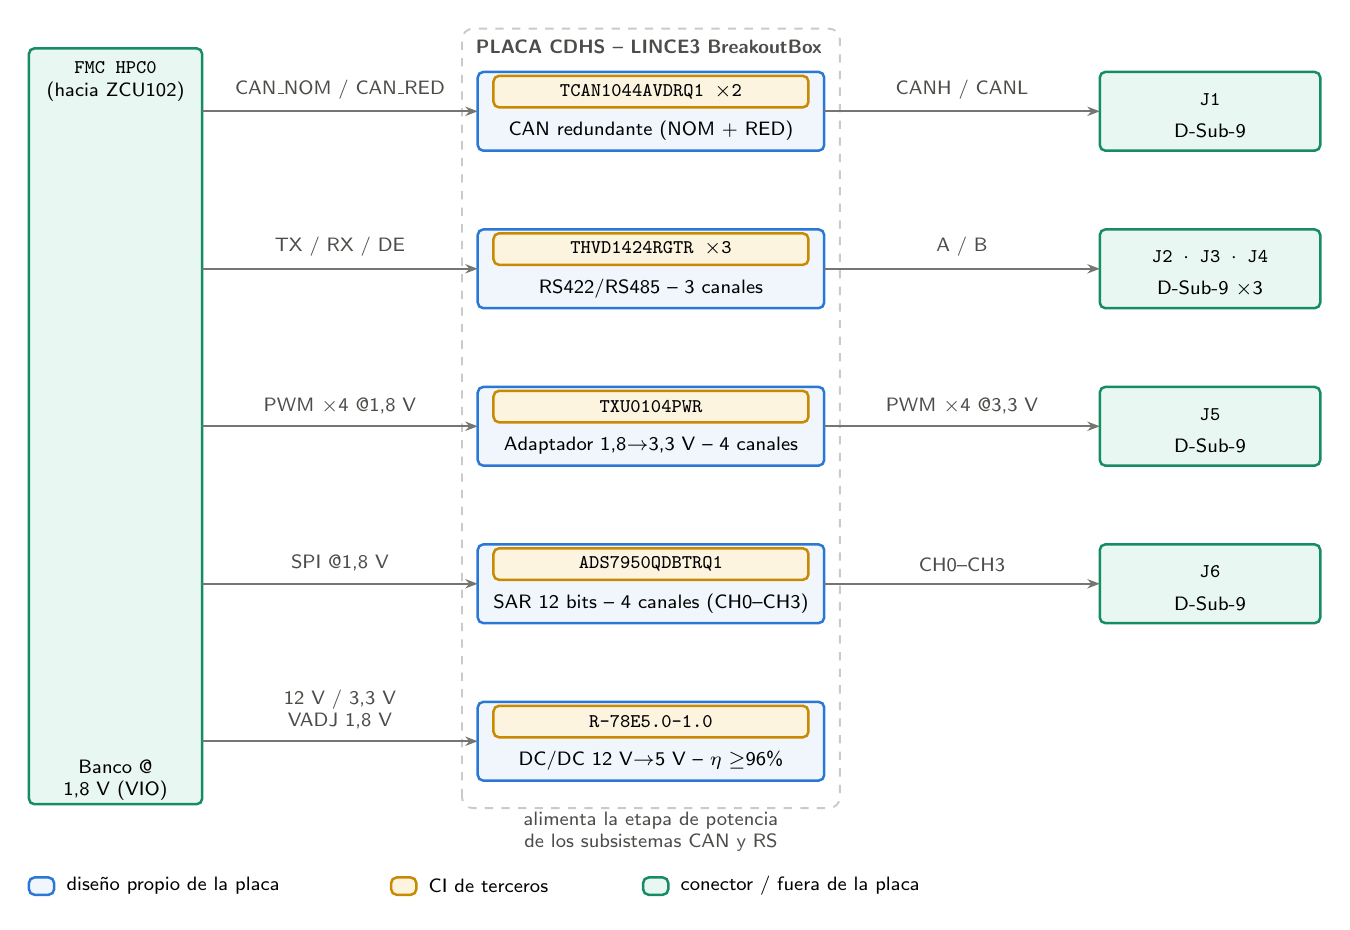
\begin{tikzpicture}[
    x=1cm, y=1cm, font=\sffamily\small,
    blk/.style={draw=cPropio, line width=0.9pt, rounded corners=2pt,
                fill=cPropio!7},
    ip/.style={draw=cIP!85!black, line width=0.9pt, rounded corners=2pt,
               fill=cIP!12},
    ext/.style={draw=cExt!80!black, line width=0.9pt, rounded corners=2pt,
                fill=cExt!10},
    band/.style={draw=cRef!45, dashed, line width=0.7pt, rounded corners=4pt},
    sig/.style={-{Stealth[length=4.5pt]}, line width=0.7pt, cRef!85!black},
    pwr/.style={-{Stealth[length=4pt]}, dashed, line width=0.6pt, cRef!70!black},
    lbl/.style={font=\sffamily\scriptsize, inner sep=2pt},
    tlbl/.style={font=\ttfamily\scriptsize, inner sep=2pt},
    name/.style={font=\ttfamily\scriptsize, align=center},
]

% ===================== Banda de la placa =====================
\draw[band] (5.50,-0.05) rectangle (10.30,9.85);
\node[lbl, anchor=north west, text=cRef!55!black] at (5.60,9.78)
      {\textbf{PLACA CDHS -- LINCE3 BreakoutBox}};

% ===================== Conector FMC (izquierda) =====================
\draw[ext] (0.00,0.00) rectangle (2.20,9.60);
\node[name] at (1.10,9.35) {FMC HPC0};
\node[lbl] at (1.10,9.05) {(hacia ZCU102)};
\node[lbl, align=center] at (1.10,0.30) {Banco @\\1,8~V (VIO)};

% ===================== Subsistema CAN =====================
\draw[blk] (5.70,8.30) rectangle (10.10,9.30);
\draw[ip] (5.90,8.85) rectangle (9.90,9.25);
\node[name] at (7.90,9.05) {TCAN1044AVDRQ1 $\times$2};
\node[lbl] at (7.90,8.55) {CAN redundante (NOM + RED)};

% ===================== Subsistema RS422/RS485 =====================
\draw[blk] (5.70,6.30) rectangle (10.10,7.30);
\draw[ip] (5.90,6.85) rectangle (9.90,7.25);
\node[name] at (7.90,7.05) {THVD1424RGTR $\times$3};
\node[lbl] at (7.90,6.55) {RS422/RS485 -- 3 canales};

% ===================== Subsistema PWM (calentadores) =====================
\draw[blk] (5.70,4.30) rectangle (10.10,5.30);
\draw[ip] (5.90,4.85) rectangle (9.90,5.25);
\node[name] at (7.90,5.05) {TXU0104PWR};
\node[lbl] at (7.90,4.55) {Adaptador 1,8$\rightarrow$3,3~V -- 4 canales};

% ===================== Subsistema ADC (termistores) =====================
\draw[blk] (5.70,2.30) rectangle (10.10,3.30);
\draw[ip] (5.90,2.85) rectangle (9.90,3.25);
\node[name] at (7.90,3.05) {ADS7950QDBTRQ1};
\node[lbl] at (7.90,2.55) {SAR 12 bits -- 4 canales (CH0--CH3)};

% ===================== Alimentación =====================
\draw[blk] (5.70,0.30) rectangle (10.10,1.30);
\draw[ip] (5.90,0.85) rectangle (9.90,1.25);
\node[name] at (7.90,1.05) {R-78E5.0-1.0};
\node[lbl] at (7.90,0.55) {DC/DC 12~V$\rightarrow$5~V -- $\eta\geq$96\%};
\node[lbl, text=cRef!55!black, align=center] at (7.90,-0.35)
      {alimenta la etapa de potencia\\de los subsistemas CAN y RS};

% ===================== Conectores externos (derecha) =====================
\draw[ext] (13.60,8.30) rectangle (16.40,9.30);
\node[name] at (15.00,8.95) {J1};
\node[lbl] at (15.00,8.55) {D-Sub-9};

\draw[ext] (13.60,6.30) rectangle (16.40,7.30);
\node[name] at (15.00,6.95) {J2 $\cdot$ J3 $\cdot$ J4};
\node[lbl] at (15.00,6.55) {D-Sub-9 $\times$3};

\draw[ext] (13.60,4.30) rectangle (16.40,5.30);
\node[name] at (15.00,4.95) {J5};
\node[lbl] at (15.00,4.55) {D-Sub-9};

\draw[ext] (13.60,2.30) rectangle (16.40,3.30);
\node[name] at (15.00,2.95) {J6};
\node[lbl] at (15.00,2.55) {D-Sub-9};

% ===================== Líneas: FMC -> subsistemas =====================
\draw[sig] (2.20,8.80) -- (5.70,8.80);
\node[lbl, anchor=south, text=cRef!55!black] at (3.95,8.88) {CAN\_NOM / CAN\_RED};

\draw[sig] (2.20,6.80) -- (5.70,6.80);
\node[lbl, anchor=south, text=cRef!55!black] at (3.95,6.88) {TX / RX / DE};

\draw[sig] (2.20,4.80) -- (5.70,4.80);
\node[lbl, anchor=south, text=cRef!55!black] at (3.95,4.88) {PWM $\times$4 @1,8~V};

\draw[sig] (2.20,2.80) -- (5.70,2.80);
\node[lbl, anchor=south, text=cRef!55!black] at (3.95,2.88) {SPI @1,8~V};

\draw[sig] (2.20,0.80) -- (5.70,0.80);
\node[lbl, anchor=south, text=cRef!55!black, align=center] at (3.95,0.88) {12~V / 3,3~V\\VADJ 1,8~V};

% ===================== Líneas: subsistemas -> conectores =====================
\draw[sig] (10.10,8.80) -- (13.60,8.80);
\node[lbl, anchor=south, text=cRef!55!black] at (11.85,8.88) {CANH / CANL};

\draw[sig] (10.10,6.80) -- (13.60,6.80);
\node[lbl, anchor=south, text=cRef!55!black] at (11.85,6.88) {A / B};

\draw[sig] (10.10,4.80) -- (13.60,4.80);
\node[lbl, anchor=south, text=cRef!55!black] at (11.85,4.88) {PWM $\times$4 @3,3~V};

\draw[sig] (10.10,2.80) -- (13.60,2.80);
\node[lbl, anchor=south, text=cRef!55!black] at (11.85,2.88) {CH0--CH3};

% ===================== Leyenda =====================
\draw[blk] (0.00,-1.15) rectangle (0.32,-0.93);
\node[lbl, anchor=west] at (0.40,-1.04) {diseño propio de la placa};
\draw[ip] (4.60,-1.15) rectangle (4.92,-0.93);
\node[lbl, anchor=west] at (5.00,-1.04) {CI de terceros};
\draw[ext] (7.80,-1.15) rectangle (8.12,-0.93);
\node[lbl, anchor=west] at (8.20,-1.04) {conector / fuera de la placa};

\end{tikzpicture}
\end{document}
